\section{Instruktionsparallelismus}
	\subsection{Superskalarität}
		Bei Superskalarität werden gleichzeitig an mehrere Recheneinheiten Befehle eines Threads geschickt, die dann parallel abgearbeitet werden. Auf Hardwareebene muss dafür die Logik der BA-Phase vervielfältigt werden: \newline
		\begin{center}
			\textbf{Pipeline mit 4 Recheneinheiten in der BA-Phase} \newline
			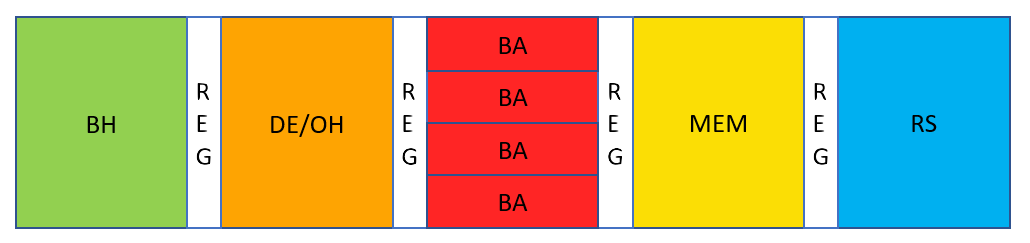
\includegraphics[scale=0.45]{Superskalare_Pipeline_mit_4_BA.png}
			\textbf{2-fach superskalare Pipeline mit 4 Recheneinheiten in der BA-Phase}\newline
			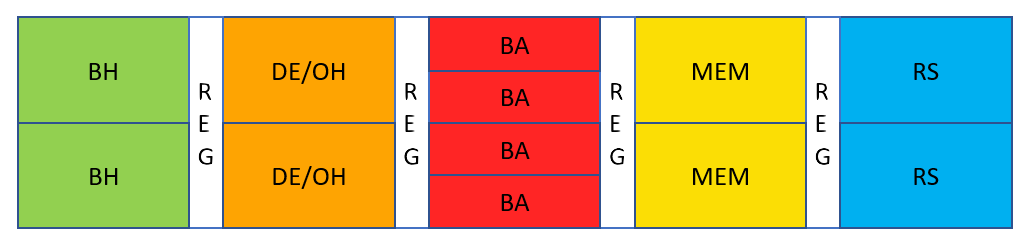
\includegraphics[scale=0.45]{2-fach_Superskalare_Pipeline_mit_4_BA.png}
		\end{center}
		\subsubsection{Dynamische Parallelisierung}
			Nicht alle Befehle eines sequentiellen Befehlsstrom können parallel ausgeführt werden. Datenhazards, also Datenabhängigkeiten zwischen Registern, sind ein Grund dafür. Bei Superskalarität wird deshalb spezielle Hardware eingefügt, die diese Abhängigkeiten erkennen und auflösen kann. \newline \newline
			Bei superskalaren Pipelines können auch Strukturhazards auftreten. Ein solcher tritt auf, wenn eine Recheneinheit (z.B. der Dividerer) benötigt wird, jedoch gerade noch durch eine andere Instruktion belegt ist. Auch für die Auflösung von Strukturhazards muss zusätzliche Hardware eingefügt werden, die die Belegung der Recheneinheiten überwacht und ggf. Befehle verzögert. \newline \newline
			Die Parallelisierung geschieht also zur Laufzeit durch die Hardware, was als dynamische Parallelisierung bezeichnet wird.
	\subsection{Very Long Instruction Word}
		Auch bei der Nutzung eines VLIW (Very Long Instruction Word) ist das Ziel die Beschleunigung der Abarbeitung von sequentiellen Programmen. Wie bei Superskalarität wird Parallelität auf Befehlsebene ausgenutzt. Im Gegensatz zur Ausführung bei Superskalarität werden die Befehle nicht dynamisch zur Laufzeit gruppiert, sondern statisch vom Compiler vor der Laufzeit. Dies wird auch als statische Parallelisierung bezeichnet \newline \newline
		Der Compiler fügt parallel ausführbare Instruktionen (ohne Datenabhängigkeiten!) zu einem Instruktionswort zusammen. Die maximal mögliche Anzahl ist dabei abhängig von der Länge des Instruktionswortes. Dieses durchläuft dann sequentiell die Pipeline: \newline
		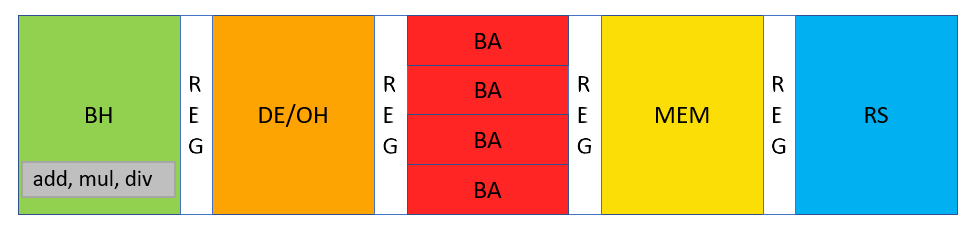
\includegraphics[scale=0.6]{VLIW_1.png}
		Wenn nicht genügend parallel ausführbare Operationen zur Verfügung stehen, muss der Compiler ein oder mehrere nop (no operation), also Platzhalter einfügen. Dadurch wird jedoch der Durchsatz verringert \newline
		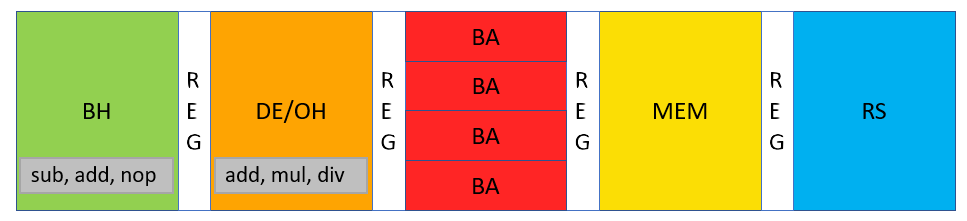
\includegraphics[scale=0.6]{VLIW_2.png} \newline
		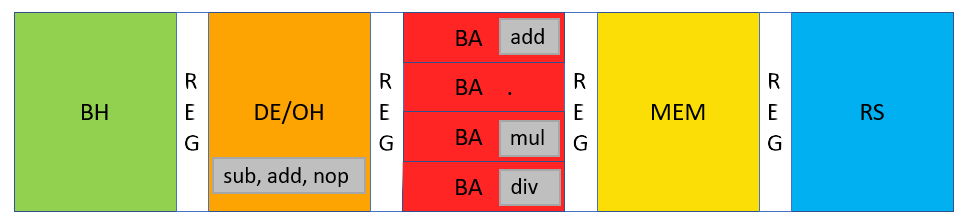
\includegraphics[scale=0.6]{VLIW_3.png}